  \chapter{Funktionen}
  \chaptertoc{}
  \cleardoubleevenpage

  \section{Der Begriff der Funktion}
      \begin{merke}
        Eine Funktion ist eine Rechenvorschrift (ein kleines Programm), welches zu einer Menge von Eingabewerten eine Ergebnismenge (Ausgabewert) erzeugt. Die Eingabewerte werden als sogenannte Parameter/Argumente an die Funktion übergeben.
      \end{merke}
      Bildlich kann man sich eine Funktion vorstellen, wie eine Maschine, an deren einem Ende etwas zugeführt wird und am Anderen entsteht ein Produkt (Ergebnis). SQL kennt zwei unterschiedliche Arten von Funktionen:
      \begin{itemize}
        \item \textbf{Single Row Functions / Skalare Funktionen}: Sie werden immer nur auf einen einzelnen Attributwert angewandt und müssen somit für jede Ergebniszeile einmal ausgeführt werden.
        \item \textbf{Grouping Functions / Aggregatfunktionen}: Diese Art von Funktionen wird pro Abfrage nur einmal ausgeführt und bezieht sich immer auf eine Gruppe von Werten (siehe \abschnitt{groupingfunctions}).
      \end{itemize}
      Die Gruppe der Single Row Functions (in SQL Server werden diese Funktionen als \enquote{Skalare Funktionen} bezeichnet) wird wiederum in mehrere Arten unterteilt.
      \begin{itemize}
        \item \textbf{Zeichenkettenfunktionen}: Dieser Funktionstyp findet Anwendung auf Zeichenketten. Mit ihm kann in Zeichenketten gesucht, Teile aus Zeichenketten herausgeschnitten und noch vieles mehr gemacht werden.
        \item \textbf{Arithmetische Funktionen}: Die Klasse der arithmetischen Funktionen führt Rechenoperationen auf den Operanden durch (z. B. Runden, Radizieren, Logarithmieren, Potenzieren, Modulo, usw.).
        \item \textbf{Datumsfunktionen}: Datumsfunktionen stehen in Zusammehang mit Datumswerten. Sie können z. B. den Wochentag zu einem Datum oder einfach nur das aktuelle Systemdatum anzeigen.
        \item \textbf{Sonstige Funktionen}: Alles was sich nicht in die oben stehenden drei Kategorien einteilen lässt, zählt zu den sonstigen Funktionen.
      \end{itemize}
      \begin{merke}
        Mit Ausnahme der \FROM-Klausel, können Single Row Functions in allen anderen Klauseln genutzt werden!
      \end{merke}
    \section{Zeichenkettenfunktionen}
      Die Kategorie der Zeichenkettenfunktionen stellt nützliche Werkzeuge zur Auswertung und Modifikation von Zeichenketten\footnote{Zeichenkette = engl. String} zur Verfügung. Mit ihrer Hilfe kann man:
      \begin{itemize}
        \item die Schreibweise eines Strings (Groß- / Kleinschreibung) verändern,
        \item die Länge einer Zeichenkette ermitteln,
        \item Leerzeichen abschneiden,
        \item Teilzeichenketten (Substrings) ausschneiden
      \end{itemize}
      und noch vieles mehr. An dieser Stelle sollen einige Beispiele für Zeichenkettenfunktionen in Oracle und SQL Server gezeigt werden.

      \begin{merke}
        Das wesentliche Ziel dieses Abschnittes ist es, dem Teilnehmer die Anwendung von Funktionen im Allgemeinen näher zu bringen. Spezielle Kenntnisse über einzelne Funktionen stehen dabei im Hintergrund.
      \end{merke}
      \subsection{Groß- oder Kleinschreibung - UPPER, LOWER, INITCAP}
        In \abschnitt{stringdiff} wurde bereits auf die Problematik der Casesensitivität hingewiesen. Oracle ist standardmässig casesensitiv, SQL Server nicht. Soll in Oracle nach einer bestimmten Zeichenkette, z. B. einem Nachnamen gesucht werden und die korrekte Schreibweise ist nicht bekannt, kann es vorkommen, dass das gewünschte Ergebnis nicht erreicht wird. Hierfür gibt es eine Lösung: Die Funktionen \languageorasql{UPPER}, \languageorasql{LOWER} und \languageorasql{INITCAP}.
        \begin{center}
          \tablecaption{Zeichenkettenfunktionen}
          \label{srfstringfct1}
          \begin{small}
            \tablefirsthead{
              \multicolumn{1}{c}{\textbf{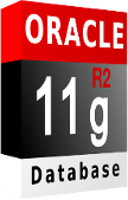
\includegraphics[scale=1]{oracle_11g}}} &
              \multicolumn{1}{c}{\textbf{
\includegraphics[scale=1]{ms_sql}}} &
              \multicolumn{1}{c}{} \\
              \multicolumn{2}{c}{\textbf{Funktionsbezeichnung}} &
              \multicolumn{1}{c}{\textbf{Bedeutung}} \\
              \hline
            }
            \tabletail{
              \hline
            }
            \tablelasttail {
              \hline
            }
            \begin{supertabular}{|c|c|p{11cm}|}
              UPPER & UPPER& Wandelt die gesamte Zeichenkette in Großbuchstaben um.\\
              \hline
              LOWER & LOWER & Wandelt die gesamte Zeichenkette in Kleinbuchstaben um.\\
              \hline
              INITCAP & n. a.& Wandelt das erste Zeichen jedes Wortes in einen Großbuchstaben um.\\
            \end{supertabular}
          \end{small}
        \end{center}
        \begin{merke}
          Die Funktion \languageorasql{INITCAP} existiert in MS SQL Server nicht!
        \end{merke}
\clearpage
        \beispiel{sql03_01} zeigt die Anwendung der drei Funktionen \languageorasql{UPPER}, \languageorasql{LOWER} und \languageorasql{INITCAP} in Oracle.
        \begin{lstlisting}[language=oracle_sql,caption={UPPER, LOWER und INITCAP},label=sql03_01]
SELECT UPPER(Vorname) AS GROSS, LOWER(Nachname) AS Klein,
       INITCAP(Vorname || ' ' || Nachname) AS NORMAL
FROM   Mitarbeiter;
        \end{lstlisting}
        \begin{center}
          \begin{small}
            \changefont{pcr}{m}{n}
            \tablefirsthead {
              \multicolumn{1}{l}{\textbf{GROSS}} &
              \multicolumn{1}{l}{\textbf{KLEIN}} &
              \multicolumn{1}{l}{\textbf{NORMAL}} \\
              \cmidrule(l){1-1}\cmidrule(l){2-2}\cmidrule(l){3-3}
            }
            \tablehead{}
            \tabletail {
            }
            \tablelasttail {
              \multicolumn{3}{l}{\textbf{100 Zeilen ausgewählt}} \\
            }
            \begin{oraclesql}
              \begin{supertabular}{lll}
                MAX & winter & Max Winter \\
                SARAH & werner & Sarah Werner \\
                FINN & seifert & Finn Seifert \\
                SEBASTIAN & schwarz & Sebastian Schwarz \\
              \end{supertabular}
            \end{oraclesql}
          \end{small}
        \end{center}
        \begin{merke}
          Die Anwendung der Funktionen \languageorasql{UPPER} und \languageorasql{LOWER} ist in Oracle und MS SQL Server identisch!
        \end{merke}
        Eingangs wurde erwähnt, das Single Row Functions nicht nur in der \SELECT-Klausel genutzt werden können, sondern, z. B. auch in der \WHERE-Klausel. Dadurch kann das beschriebene Problem der Casesensitivität gelöst werden.
        \begin{lstlisting}[language=oracle_sql,caption={Das Problem der Casesensitivität},label=sql03_02]
SELECT Mitarbeiter_ID, Vorname, Nachname
FROM   Mitarbeiter
WHERE  Nachname LIKE 'winter';
        \end{lstlisting}
        \begin{center}
          \begin{small}
            \changefont{pcr}{m}{n}
            \tablefirsthead {
              \multicolumn{1}{r}{\textbf{MITARBEITER\_ID}} &
              \multicolumn{1}{l}{\textbf{VORNAME}} &
              \multicolumn{1}{l}{\textbf{NACHNAME}} \\
              \cmidrule(r){1-1}\cmidrule(l){2-2}\cmidrule(l){3-3}
            }
            \tablehead{}
            \tabletail {
              \multicolumn{3}{l}{\textbf{Keine Zeilen ausgewählt}} \\
            }
            \tablelasttail {
              \multicolumn{3}{l}{\textbf{Keine Zeilen ausgewählt}} \\
            }
            \begin{oraclesql}
              \begin{supertabular}{rll}

              \end{supertabular}
            \end{oraclesql}
          \end{small}
        \end{center}
        Der Mitarbeiter \enquote{Winter} wird von Oracle nicht gefunden, da er in der Datenbank mit einem großen W am Namensanfang gespeichert ist. Für Oracle sind \enquote{winter} und \enquote{Winter} zwei unterschiedliche Zeichenketten. Hier kann die \languageorasql{LOWER}-Funktion Abhilfe schaffen.
        \begin{lstlisting}[language=oracle_sql,caption={LOWER - Die Lösung des Problems},label=sql03_03]
SELECT Mitarbeiter_ID, Vorname, Nachname
FROM   Mitarbeiter
WHERE  LOWER(Nachname) LIKE 'winter';
        \end{lstlisting}
\clearpage
        \begin{center}
          \begin{small}
            \changefont{pcr}{m}{n}
            \tablefirsthead {
              \multicolumn{1}{r}{\textbf{MITARBEITER\_ID}} &
              \multicolumn{1}{l}{\textbf{VORNAME}} &
              \multicolumn{1}{l}{\textbf{NACHNAME}} \\
              \cmidrule(r){1-1}\cmidrule(l){2-2}\cmidrule(l){3-3}
            }
            \tablehead{}
            \tabletail {
              \multicolumn{3}{l}{\textbf{2 Zeilen ausgewählt}} \\
            }
            \tablelasttail {
              \multicolumn{3}{l}{\textbf{2 Zeilen ausgewählt}} \\
            }
            \begin{oraclesql}
              \begin{supertabular}{rll}
                1 & Max & Winter \\
                9 & Louis & Winter \\
              \end{supertabular}
            \end{oraclesql}
          \end{small}
        \end{center}
        Die \languageorasql{LOWER}-Funktion stellt in \beispiel{sql03_03} sicher, dass alle Werte der Spalte \identifier{Nachname} in Kleinbuchstaben ausgegeben werden. Somit ist der Vergleich mit \enquote{winter} unproblematisch.
      \subsection{Zeichenketten bearbeiten}
        Eine weitere Anwendung von Zeichenkettenfunktionen besteht darin, Teile aus Zeichenketten herauszutrennen oder deren Länge festzustellen. Hierzu kennen Oracle und SQL Server unterschiedliche Funktionen, die in \tabelle{srfstringfct2} beschrieben werden. Sie stellt jedoch nur einen Ausschnitt aus der Menge der Zeichenkettenfunktionen dar.
        \begin{center}
          \tablecaption{Zeichenkettenfunktionen}
          \label{srfstringfct2}
          \begin{small}
            \tablefirsthead{
              \multicolumn{1}{c}{\textbf{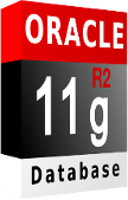
\includegraphics[scale=1]{oracle_11g}}} &
              \multicolumn{1}{c}{\textbf{
\includegraphics[scale=1]{ms_sql}}} &
              \multicolumn{1}{c}{} \\
              \multicolumn{2}{c}{\textbf{Funktionsbezeichnung}} &
              \multicolumn{1}{c}{\textbf{Bedeutung}} \\
              \hline
            }
            \tabletail{
              \hline
            }
            \tablelasttail {
              \hline
            }
            \begin{supertabular}{|l|l|p{10cm}|}
              SUBSTR & SUBSTRING &  Schneidet einen Teil einer Zeichenkette aus und liefert ihn zurück. \\
              \hline
              LENGTH & LEN &  Gibt die Länge einer Zeichenkette zurück. \\
              \hline
              INSTR & CHARINDEX & Diese Funktionen suchen nach Zeichenkette A in
              einer Zeichenkette B und liefern die Position von A zurück. Ist
              A nicht in B erhält man 0 als Ergebnis. \\
            \end{supertabular}
          \end{small}
        \end{center}
        \subsubsection{SUBSTR, LENGTH und INSTR in Oracle}
          Die Funktion \languageorasql{LENGTH} ermittelt, aus wie vielen Zeichen
          ein String besteht. Sie wird meist in Zusammenhang mit den beiden
          anderen Funktionen \languageorasql{SUBSTR} und \languageorasql{INSTR}
          genutzt. \beispiel{sql03_04} zeigt die Anwendung von
          \languageorasql{LENGTH} auf sehr einfache Art und Weise.
          \begin{lstlisting}[language=oracle_sql,caption={Die \languageorasql{LENGTH}-Funktion},label=sql03_04]
SELECT LENGTH(IBAN), IBAN
FROM   Konto
WHERE  Konto_ID = 1281;
          \end{lstlisting}
          \begin{center}
            \begin{small}
              \changefont{pcr}{m}{n}
              \tablefirsthead {
                \multicolumn{1}{r}{\textbf{LENGTH(IBAN)}} &
                \multicolumn{1}{l}{\textbf{IBAN}} \\
                \cmidrule(r){1-1}\cmidrule(l){2-2}
              }
              \tablehead{}
              \tabletail {
%                 \multicolumn{2}{l}{\textbf{1 Zeile ausgewählt}} \\
              }
              \tablelasttail {
                \multicolumn{2}{l}{\textbf{1 Zeile ausgewählt}} \\
              }
              \begin{oraclesql}
                \begin{supertabular}{rl}
                  22 & DE23465387306148533897 \\
                \end{supertabular}
              \end{oraclesql}
            \end{small}
          \end{center}
          Alleine für sich, ist die Information \enquote{22} auf den ersten Blick nutzlos, wenn man aber bedenkt, dass z. B. eine IBAN eine feste Länge von 22 Zeichen hat, kann man mit Hilfe von \languageorasql{LENGTH} verifizieren, ob es sich um eine IBAN mit
          gültiger Länge handelt.

          \languageorasql{SUBSTR} ist dabei behilflich, einen Teil aus einer Zeichenkette auszuschneiden. Eine solche Vorgehensweise ist z. B. dann notwendig, wenn eine Information, in der Form \enquote{Winter, Max}, in einer Tabellenspalte abgelegt ist oder, wenn wie im Falle der IBAN, mehrere Informationen einfach verkettet wurden (Länderkennung, Prüfziffer, BLZ und KtoNr).

          \begin{merke}
            Das Ergebnis einer solchen Operation wird als \enquote{Teilzeichenkette} oder \enquote{Substring} bezeichnet, wobei \enquote{Substring} die geläufigere Variante darstellt.
          \end{merke}
          \beispiel{sql03_05} zeigt die Anwendung der Funktion \languageorasql{SUBSTR}, um die IBAN eines Kontos in ihre Bestandteile zu zerlegen. Hier kann für den dritten wert der Funktion auch eine andere Funktion mit angegeben werden.
          \begin{lstlisting}[language=oracle_sql,caption={Die Anwendung der Funktion \languageorasql{SUBSTR}},label=sql03_05]
SELECT SUBSTR(IBAN, 1, 2) AS Laenderkuerzel, SUBSTR(IBAN, 5 , 8) AS BLZ,
       SUBSTR(IBAN, 13, LEN(IBAN)) AS KtoNr
FROM   Konto
WHERE  Konto_ID = 1281;
          \end{lstlisting}
          \begin{center}
            \begin{small}
              \changefont{pcr}{m}{n}
              \tablefirsthead {
                \multicolumn{1}{l}{\textbf{LAENDE}} &
                \multicolumn{1}{l}{\textbf{BLZ}} &
                \multicolumn{1}{l}{\textbf{KTONR}} \\
                \cmidrule(l){1-1}\cmidrule(l){2-2}\cmidrule(l){3-3}
              }
              \tablehead{}
              \tabletail {
                \multicolumn{2}{l}{\textbf{1 Zeile ausgewählt}} \\
              }
              \tablelasttail {
                \multicolumn{2}{l}{\textbf{1 Zeile ausgewählt}} \\
              }
              \begin{oraclesql}
                \begin{supertabular}{lrr}
                  DE & 46538730 & 6148533897 \\
                \end{supertabular}
              \end{oraclesql}
            \end{small}
          \end{center}
          \begin{center}
            \tablecaption{Funktionsargumente von SUBSTR}
            \label{argsubstr}
            \begin{small}
              \tablefirsthead{
                \multicolumn{1}{c}{\textbf{Argument}} &
                \multicolumn{1}{c}{\textbf{Beispiel}} &
                \multicolumn{1}{c}{\textbf{Erläuterung}} \\
                \hline
              }
              \tablehead{}
              \tabletail{
                \hline
              }
              \tablelasttail{
                \hline
              }
              \begin{supertabular}{|l|c|p{8.5cm}|}
                1 & IBAN &
                Beliebige Zeichenkette (Literal, Spaltenbezeichner oder eine
                andere Funktion). \\
                \hline
                2 & 11 & An welcher Stelle im ersten Argument soll das
                Ausschneiden begonnen werden?. Hier kann eine beliebige
                Integerzahl stehen, die kleiner ist, als die Gesamtlänge von Argument 1. \\
                \hline
                3 & 16 & Mit dem dritten und letzten Argument wird angegeben,
                wie viele Zeichen ausgeschnitten werden sollen.
                \begin{itemize}
                  \item n > 1: Es werden n Zeichen ausgeschnitten.
                  \item n nicht angegeben: Es werden alle Zeichen, bis zum Ende der Zeichenkette angezeigt.
                  \item n < 1: NULL-Wert als Ergebnis
                \end{itemize} \\
              \end{supertabular}
            \end{small}
          \end{center}

          Mit \languageorasql{INSTR} kann die Position eines Zeichens oder einer
          Zeichenkette in einer Zeichenkette bestimmt werden. Eine typische
          Aufgabenstellung könnte sein: \enquote{Bestimme ob das
          Länderkürzel DE in der IBAN vorkommt}.
          In SQL ausgedrückt sieht dies so aus:
          \begin{lstlisting}[language=oracle_sql,caption={Automatische Positionsbestimmung},label=sql03_06]
SELECT INSTR(IBAN, 'DE') AS Position
FROM   Konto
WHERE  Konto_ID = 1281;
          \end{lstlisting}
          \begin{center}
            \begin{small}
              \changefont{pcr}{m}{n}
              \tablefirsthead {
                \multicolumn{1}{r}{\textbf{POSITION}} \\
                \cmidrule(r){1-1}
              }
              \tablehead{}
              \tabletail {
                \multicolumn{1}{l}{\textbf{1 Zeile ausgewählt}} \\
              }
              \tablelasttail {
                \multicolumn{1}{l}{\textbf{1 Zeile ausgewählt}} \\
              }
              \begin{oraclesql}
                \begin{supertabular}{r}
                  1 \\
                \end{supertabular}
              \end{oraclesql}
            \end{small}
          \end{center}
          \beispiel{sql03_06} zeigt, wie mit Hilfe der
          \languageorasql{INSTR}-Funktion die Position eines einzelnen Zeichens
          bzw. mehrere Zeichen in einer Zeichenkette ermittelt werden kann.
          \begin{center}
            \tablecaption{Funktionsargumente von INSTR}
            \label{arginstr}
            \begin{small}
              \tablefirsthead{
                \multicolumn{1}{c}{\textbf{Argument}} &
                \multicolumn{1}{c}{\textbf{Beispiel}} &
                \multicolumn{1}{c}{\textbf{Erläuterung}} \\
                \hline
              }
              \tablehead{}
              \tabletail{
                \hline
              }
              \tablelasttail{
                \hline
              }
              \begin{supertabular}{|l|c|p{8.5cm}|}
                1 & IBAN &
                Beliebige Zeichenkette (Literal, Spaltenbezeichner oder eine
                andere Funktion). \\
                \hline
                2 & 'DE' & Das zweite Argument gibt an, nach welchem Zeichen /
                welcher Zeichenkette gesucht werden soll. \\
              \end{supertabular}
            \end{small}
          \end{center}
          \begin{merke}
            Die Funktion \languageorasql{INSTR} kennt noch zwei weitere
            Parameter, welche hier nicht näher erläutert werden. Weitere
            Informationen zu dieser Funktion können aus der
            Online-Dokumentation entnommen werden.
          \end{merke}
          Die folgenden Links verweisen auf die Online-Dokumentation der
          Oracle-Datenbank.
          \begin{literaturinternet}
            \item \cite{i77725}
            \item \cite{i87066}
            \item \cite{i77598}
          \end{literaturinternet}
\clearpage
        \subsubsection{SUBSTRING, LEN und CHARINDEX in MS SQL Server}
          Die Funktion \languagemssql{LEN} ermittelt, aus wie vielen Zeichen ein
          String besteht. Sie wird meist in Zusammenhang mit den beiden anderen
          Funktionen \languagemssql{SUBSTRING} und \languagemssql{CHARINDEX}
          genutzt. \beispiel{sql03_08} zeigt die Anwendung von
         \languagemssql{LEN} auf sehr einfache Art und Weise.
          \begin{lstlisting}[language=ms_sql,caption={Die \languagemssql{LEN}-Funktion},label=sql03_08]
SELECT LEN(IBAN), IBAN
FROM   Konto
WHERE  Konto_ID = 1281;
          \end{lstlisting}
          \begin{center}
            \begin{small}
              \changefont{pcr}{m}{n}
              \tablefirsthead {
                \multicolumn{1}{l}{\textbf{(Kein Spaltenname)}} &
                \multicolumn{1}{l}{\textbf{Nachname}} \\
                \cmidrule(l){1-1}\cmidrule(l){2-2}
              }
              \tablehead{}
              \tabletail {
                \multicolumn{2}{l}{\textbf{1 Zeile ausgewählt}} \\
              }
              \tablelasttail {
                \multicolumn{2}{l}{\textbf{1 Zeile ausgewählt}} \\
              }
              \begin{mssql}
                \begin{supertabular}{ll}
                  22 & DE23465387306148533897 \\
                \end{supertabular}
              \end{mssql}
            \end{small}
          \end{center}
          Alleine für sich, ist die Information \enquote{22} auf den
          ersten Blick nutzlos, wenn man aber bedenkt, dass z. B. eine IBAN
          eine feste Länge von 22 Zeichen hat, kann man mit Hilfe von
          \languagemssql{LEN} verifizieren, ob es sich um eine IBAN mit
          gültiger Länge handelt.

          \languagemssql{SUBSTRING} ist dabei behilflich, einen Teil aus einer Zeichenkette auszuschneiden. Eine solche Vorgehensweise ist z. B. dann notwendig, wenn eine Information, in der Form \enquote{Winter, Max}, in einer Tabellenspalte abgelegt ist oder, wenn wie im Falle der IBAN, mehrere Informationen einfach verkettet wurden (Länderkennung, Prüfziffer, BLZ und KtoNr).

          \begin{merke}
            Das Ergebnis einer solchen Operation wird als \enquote{Teilzeichenkette} oder \enquote{Substring} bezeichnet, wobei \enquote{Substring} die geläufigere Variante darstellt.
          \end{merke}
          \beispiel{sql03_09} zeigt die Anwendung der Funktion \languagemssql{SUBSTRING}, um die IBAN eines Kontos in ihre Bestandteile zu zerlegen.
          \begin{lstlisting}[language=ms_sql,caption={Die Anwendung der Funktion \languagemssql{SUBSTRING}},label=sql03_09]
SELECT SUBSTRING(IBAN, 1, 2) AS Laenderkuerzel, SUBSTRING(IBAN, 5 , 8) AS BLZ,
       SUBSTRING(IBAN, 14) AS KtoNr
FROM   Konto
WHERE  Konto_ID = 1281;
          \end{lstlisting}
\clearpage
          \begin{center}
            \begin{small}
              \changefont{pcr}{m}{n}
              \tablefirsthead {
                \multicolumn{1}{l}{\textbf{LAENDE}} &
                \multicolumn{1}{l}{\textbf{BLZ}} &
                \multicolumn{1}{l}{\textbf{KTONR}} \\
                \cmidrule(l){1-1}\cmidrule(l){2-2}\cmidrule(l){3-3}
              }
              \tablehead{}
              \tabletail {
                \multicolumn{2}{l}{\textbf{1 Zeile ausgewählt}} \\
              }
              \tablelasttail {
                \multicolumn{2}{l}{\textbf{1 Zeile ausgewählt}} \\
              }
              \begin{mssql}
                \begin{supertabular}{lll}
                  DE & 46538730 & 6148533897 \\
                \end{supertabular}
              \end{mssql}
            \end{small}
          \end{center}
          \begin{center}
            \tablecaption{Funktionsargumente von SUBSTR}
            \label{argSUBSTRING}
            \begin{small}
              \tablefirsthead{
                \multicolumn{1}{c}{\textbf{Argument}} &
                \multicolumn{1}{c}{\textbf{Beispiel}} &
                \multicolumn{1}{c}{\textbf{Erläuterung}} \\
                \hline
              }
              \tablehead{}
              \tabletail{
                \hline
              }
              \tablelasttail{
                \hline
              }
              \begin{supertabular}{|l|c|p{8.5cm}|}
                1 & IBAN &
                Beliebige Zeichenkette (Literal, Spaltenbezeichner oder eine
                andere Funktion). \\
                \hline
                2 & 11 & An welcher Stelle im ersten Argument soll das
                Ausschneiden begonnen werden?. Hier kann eine beliebige
                Integerzahl stehen, die kleiner ist, als die Gesamtlänge von Argument 1. \\
                \hline
                3 & 16 & Mit dem dritten und letzten Argument wird angegeben,
                wie viele Zeichen ausgeschnitten werden sollen.
                \begin{itemize}
                  \item n > 1: Es werden n Zeichen ausgeschnitten.
                  \item n nicht angegeben: Es werden alle Zeichen, bis zum Ende der Zeichenkette angezeigt.
                  \item n < 1: NULL-Wert als Ergebnis
                \end{itemize} \\
              \end{supertabular}
            \end{small}
          \end{center}
          Mit \languagemssql{CHARINDEX} kann die Position eines Zeichens oder
          einer Zeichenkette in einer Zeichenkette bestimmt werden. Eine
          typische Aufgabenstellung könnte sein: \enquote{Bestimme ob das
          Länderkürzel DE in der IBAN vorkommt}. In SQL ausgedrückt sieht dies so aus:
          \begin{lstlisting}[language=ms_sql,caption={Automatische Positionsbestimmung},label=sql03_10]
SELECT CHARINDEX('DE', IBAN) AS Position
FROM   Konto
WHERE  Konto_ID = 1281;
          \end{lstlisting}

          \begin{center}
            \begin{small}
              \changefont{pcr}{m}{n}
              \tablefirsthead {
                \multicolumn{1}{l}{\textbf{POSITION}} \\
                \cmidrule(r){1-1}
              }
              \tablehead{}
              \tabletail {
                \multicolumn{1}{l}{\textbf{1 Zeile ausgewählt}} \\
              }
              \tablelasttail {
                \multicolumn{1}{l}{\textbf{1 Zeile ausgewählt}} \\
              }
              \begin{mssql}
                \begin{supertabular}{l}
                  1 \\
                \end{supertabular}
              \end{mssql}
            \end{small}
          \end{center}
          \beispiel{sql03_10} zeigt, wie mit Hilfe der
          \languagemssql{CHARINDEX}-Funktion die Position eines einzelnen
          Zeichens in einer Zeichenkette ermittelt werden kann.
          \begin{center}
            \tablecaption{Funktionsargumente von CHARINDEX}
            \label{argcharindex}
            \begin{small}
              \tablefirsthead{
                \multicolumn{1}{c}{\textbf{Argument}} &
                \multicolumn{1}{c}{\textbf{Beispiel}} &
                \multicolumn{1}{c}{\textbf{Erläuterung}} \\
                \hline
              }
              \tablehead{}
              \tabletail{
                \hline
              }
              \tablelasttail{
                \hline
              }
              \begin{supertabular}{|l|c|p{8.5cm}|}
                1 & 'DE' & Das erste Argument gibt an, nach welchem Zeichen /
                welcher Zeichenkette gesucht werden soll. \\
                \hline
                2 & Nachname + ', ' + Vorname & Das zwei Argument ist eine
                beliebige Zeichenkette. An dieser Stelle kann ein Literal, ein
                Spaltenbezeichner oder eine andere Funktion stehen. \\
                \hline
              \end{supertabular}
            \end{small}
          \end{center}
          \begin{merke}
            Die Funktion \languagemssql{CHARINDEX} kennt noch einen weiteren
            Parameter, welcher hier nicht näher erläutert wird. Weitere
            Informationen zu dieser Funktion können aus der
            Online-Dokumentation, der MSDN, entnommen werden.
          \end{merke}
          Die folgenden Links verweisen auf die Online-Dokumentation des MS SQL
          Server, im Microsoft Developer Network (MSDN).
          \begin{literaturinternet}
            \item \cite{ms190329}
            \item \cite{ms187748}
            \item \cite{ms186323}
          \end{literaturinternet}
    \section{Arithmetische Funktionen}
      Arithmetische Funktionen dienen dazu Berechnungen anzustellen. Dies kann
      beispielsweise sein:
      \begin{itemize}
        \item Runden,
        \item Radizieren (Wurzelziehen),
        \item Potenzieren,
        \item Logarithmieren
      \end{itemize}
      und vieles mehr. In dieser Unterrichtsunterlage werden nur einige
      Beispiele gezeigt.
      \subsection{FROM oder nicht FROM, das ist hier die Frage}
        In \beispiel{sql03_12} und \beispiel{sql03_13} wird die Berechnung der
        Quadratwurzel, der Zahl 4, in Oracle und MS SQL Server gezeigt. Die
        Anwendung der Funktion \languageorasql{SQRT} ist in beiden Systemen
        gleich. Trotztdem existiert ein gravierender Unterschied zwischen beiden
        Beispielen.
        \begin{lstlisting}[language=oracle_sql,caption={Berechnung der Quadartwurzel, der Zahl 4, in Oracle},label=sql03_12]
SELECT SQRT(4) AS "Wurzel 4"
FROM   dual;
        \end{lstlisting}
\clearpage
        \begin{lstlisting}[language=ms_sql,caption={Berechnung der Quadratwurzel, der Zahl 4, in MS SQL Server},label=sql03_13]
SELECT SQRT(4) As "Wurzel 4";
        \end{lstlisting}
        \begin{center}
          \begin{small}
            \changefont{pcr}{m}{n}
            \tablefirsthead {
              \multicolumn{1}{r}{\textbf{Wurzel 4}} \\
              \cmidrule(r){1-1}
            }
            \tablehead{}
            \tabletail {
              \multicolumn{1}{l}{\textbf{1 Zeile ausgewählt}} \\
            }
            \tablelasttail {
              \multicolumn{1}{l}{\textbf{1 Zeile ausgewählt}} \\
            }
            \begin{msoraclesql}
              \begin{supertabular}{r}
                2 \\
              \end{supertabular}
            \end{msoraclesql}
          \end{small}
        \end{center}
        Eingangs wurde behauptet, dass jedes \SELECT-Statement immer eine
        \FROM-Klausel benötigen würde. Dies ist gemäß SQL-Standard
        auch richtig. Das DBMS Oracle setzt an dieser Stelle den Standard
        konsequent um, der MS SQL Server nicht.

        \begin{merke}
          Im DBMS Oracle muss jedes \SELECT-Statement immer eine \FROM-Klausel
          aufweisen, in MS SQL Server nicht.
        \end{merke}
			 Um den SQL-Standard einhalten zu können, gibt es in Oracle eine \enquote{Dummy-Tabelle} namens \identifier{dual}. Diese enthält nur eine 		 Spalte, mit einer Zeile, wie in \beispiel{sql03_14} zu sehen ist. Sie kommt immer dann zum Einsatz, wenn das Ergebnis einer Funktion, unabhängig von irgendwelchen Datensätzen, abgerufen werden muss.
        \begin{lstlisting}[language=oracle_sql,caption={Die Tabelle \identifier{dual} in Oracle},label=sql03_14]
SELECT *
FROM   dual;
        \end{lstlisting}
        \begin{center}
          \begin{small}
            \changefont{pcr}{m}{n}
            \tablefirsthead {
              \multicolumn{1}{l}{\textbf{DUMMY}} \\
              \cmidrule(l){1-1}
            }
            \tablehead{}
            \tabletail {
              \multicolumn{1}{l}{\textbf{1 Zeile ausgewählt}} \\
            }
            \tablelasttail {
              \multicolumn{1}{l}{\textbf{1 Zeile ausgewählt}} \\
            }
            \begin{oraclesql}
              \begin{supertabular}{l}
                X \\
              \end{supertabular}
            \end{oraclesql}
          \end{small}
        \end{center}
        Der MS SQL Server kommt ohne diese Tabelle aus, da bei ihm die
        \FROM-Klausel einfach weggelassen werden darf.
      \subsection{Arithmetische Funktionen anwenden}
        Oracle kennt ca. 30 und MS SQL Server ca. 20 arithmetische Funktionen.
        Ziel dieser Unterrichtsunterlage ist es, einige wenige davon
        herauszugreifen und deren Anwendung zu erläutern. Hierbei handelt es
        sich um die folgenden Funktionen:
\clearpage
        \begin{center}
          \tablecaption{Arithmetische Funktionen}
          \label{srfarithmfct}
          \begin{small}
            \tablefirsthead{
              \multicolumn{1}{c}{\textbf{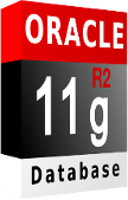
\includegraphics[scale=1]{oracle_11g}}} &
              \multicolumn{1}{c}{\textbf{
\includegraphics[scale=1]{ms_sql}}} &
              \multicolumn{1}{c}{} \\
              \multicolumn{2}{c}{\textbf{Funktionsbezeichnung}} &
              \multicolumn{1}{c}{\textbf{Bedeutung}} \\
              \hline
            }
            \tabletail{
              \hline
            }
            \tablelasttail {
              \hline
            }
            \begin{supertabular}{|l|l|p{10cm}|}
              CEIL & CEILING & Gibt immer die kleinste ganze Zahl aus, die
              größer oder gleich n ist (Ganzzahliges Aufrunden).\\
              \hline
              FLOOR & FLOOR & Gibt immer die größte ganze Zahl aus, die
              kleiner oder gleich n ist (Ganzzahliges Abrunden). \\
              \hline
              LOG & LOG 10 & Berechnet den Logarithmus der Zahl x zur Basis n. MS-SQL nur zur Basis 10 \\
              \hline
              MOD & \% & Gibt den Rest einer ganzzahligen Division zurück. \\
              \hline
              POWER & POWER & Potenziert die Zahl x mit n. \\
              \hline
              ROUND & ROUND & Auf- bzw. Abrunden einer Zahl nach dem
              kaufmännischen Rundungsverfahren ($x < 0,5$ = Abrunden, $x \geqq
              0,5$ = Aufrunden). \\
              \hline
              TRUNC & n. a. & Schneidet die Nachkommastellen einer Zahl ab und
              gibt den ganzzahligen Anteil zurück. \\
            \end{supertabular}
          \end{small}
        \end{center}
        In den beiden folgenden Beispielen wird die Anwendung von
        Rundungsfunktionen in Oracle und MS SQL Server gezeigt.
        \begin{lstlisting}[language=oracle_sql,caption={Rundungsfunktionen in Oracle},label=sql03_15]
SELECT SQRT(3) AS "Wurzel 3", CEIL(SQRT(3)) AS "Aufrunden",
       FLOOR(SQRT(3)) AS "Abrunden",
       ROUND(SQRT(3), 2) AS "Kaufm. runden"
FROM   dual;
        \end{lstlisting}
        \begin{center}
          \begin{small}
            \changefont{pcr}{m}{n}
            \tablefirsthead {
              \multicolumn{1}{r}{\textbf{Wurzel 3}} &
              \multicolumn{1}{r}{\textbf{Aufrunden}} &
              \multicolumn{1}{r}{\textbf{Abrunden}} &
              \multicolumn{1}{r}{\textbf{Kaufm. runden}} \\
              \cmidrule(r){1-1}\cmidrule(r){2-2}\cmidrule(r){3-3}\cmidrule(r){4-4}
            }
            \tablehead{}
            \tabletail {
              \multicolumn{4}{l}{\textbf{1 Zeile ausgewählt}} \\
            }
            \tablelasttail {
              \multicolumn{4}{l}{\textbf{1 Zeile ausgewählt}} \\
            }
            \begin{oraclesql}
              \begin{supertabular}{rrrr}
                1,7320508 & 2 & 1 & 1,73 \\
              \end{supertabular}
            \end{oraclesql}
          \end{small}
        \end{center}
        Die Funktionen aus \beispiel{sql03_15} sind weitestgehend
        selbsterklärend. Die mit \languageorasql{SQRT(3)} erzeugte Zahl
        1,7320508 wird durch \languageorasql{CEIL} aufgerundet auf 2, von
        \languageorasql{FLOOR} abgerundet auf 1 und mit Hilfe von
        \languageorasql{ROUND} kaufmännisch, auf zwei Nachkommastellen,
        aufgerundet.

        \begin{merke}
          Die Funktion \languageorasql{ROUND} rundet kaufmännisch. Das zweite
          Argument gibt an, auf welche Nachkommastelle gerundet werden soll.
          Durch die Angabe von 0 wird auf die nächste ganze Zahl gerundet.
        \end{merke}
        Die Anwendung dieser Funktionen ist im MS SQL Server identisch, mit der
        Ausnahme das \languageorasql{CEIL} dort \languagemssql{CEILING}
        heißt.
\clearpage
        \begin{lstlisting}[language=ms_sql,caption={Rundungsfunktionen in MS SQL},label=sql03_16]
SELECT SQRT(3) AS "Wurzel 3", CEILING(SQRT(3)) AS "Aufrunden",
       FLOOR(SQRT(3)) AS "Abrunden",
       ROUND(SQRT(3), 2) AS "Kaufm. runden";
        \end{lstlisting}
        \begin{center}
          \begin{small}
            \changefont{pcr}{m}{n}
            \tablefirsthead {
              \multicolumn{1}{l}{\textbf{Wurzel 3}} &
              \multicolumn{1}{l}{\textbf{Aufrunden}} &
              \multicolumn{1}{l}{\textbf{Abrunden}} &
              \multicolumn{1}{l}{\textbf{Kaufm. runden}} \\
              \cmidrule(l){1-1}\cmidrule(l){2-2}\cmidrule(l){3-3}\cmidrule(l){4-4}
            }
            \tablehead{}
            \tabletail {
              \multicolumn{4}{l}{\textbf{1 Zeile ausgewählt}} \\
            }
            \tablelasttail {
              \multicolumn{4}{l}{\textbf{1 Zeile ausgewählt}} \\
            }

            \begin{mssql}
              \begin{supertabular}{llll}
                1,7320508 & 2 & 1 & 1,73 \\
              \end{supertabular}
            \end{mssql}
          \end{small}
        \end{center}
        In \beispiel{sql03_15} bzw. \beispiel{sql03_16} ist zu sehen, dass es
        möglich ist, Funktionen in einander zu verschachteln. Mit Hilfe des
        Ausdrucks \languageorasql{SQRT(3)} wird die Quadratwurzel der Zahl 3
        errechnet (1,73205080756888). Dieser Wert soll anschließend auf 2
        Nachkommastellen gerundet werden. Hierzu kann auf beiden Systemen die
        Funktion \languageorasql{ROUND} herangezogen werden. 
        
        Bei der Abarbeitung des Ausdrucks \languageorasql{ROUND(SQRT(3),2)}
        halten sich Oracle und SQL Server an die Gesetze der Arithmetik, d. h.
        es wird zuerst der innerste Ausdruck (in diesem Falle
        \languageorasql{SQRT(3)}) aufgelöst und anschließend wird das
        Ergebnis dieses Ausdrucks durch die Funktion \languageorasql{ROUND} auf
        zwei Nachkommastellen gerundet.

        Die zweite Gruppe der arithmetischen Funktionen, die hier vorgestellt
        werden sollen, bilden die sogenannten \enquote{höhreren Rechenarten}
        ab. Dies sind: Radizieren, Potenzieren, Logarithmieren. Zusätzlich ist
        hier noch die Modulo-Operation dargestellt, die den Rest einer
        ganzzahlingen Divison ausgibt.
        \begin{lstlisting}[language=oracle_sql,caption={Höhere Rechenarten in Oracle},label=sql03_17]
SELECT MOD(9, 2) AS Modulo, POWER(10, 2) AS Power,
       LOG(10, 1000) AS Log, SQRT(16) AS Quadratwurzel,
       SQRT(27) / SQRT(3) AS "3. Wurzel von 27",
       LOG(5, 8) AS "Log 8 Basis 5"
FROM   dual;
        \end{lstlisting}
        \begin{center}
          \begin{small}
            \changefont{pcr}{m}{n}
            \tablefirsthead {
              \multicolumn{1}{r}{\textbf{Modulo}} &
              \multicolumn{1}{r}{\textbf{Power}} &
              \multicolumn{1}{r}{\textbf{Log}} &
              \multicolumn{1}{r}{\textbf{Quadratwurzel}} &
              \multicolumn{1}{r}{\textbf{3. Wurzel von 27}} &
              \multicolumn{1}{r}{\textbf{Log 8 Basis 5}} \\
              \cmidrule(r){1-1}\cmidrule(r){2-2}\cmidrule(r){3-3}\cmidrule(r){4-4}\cmidrule(r){5-5}
              \cmidrule(r){6-6}
            }
            \tablehead{}
            \tabletail {
              \multicolumn{6}{l}{\textbf{1 Zeile ausgewählt}} \\
            }
            \tablelasttail {
              \multicolumn{6}{l}{\textbf{1 Zeile ausgewählt}} \\
            }
            \begin{oraclesql}
              \begin{supertabular}{rrrrrr}
                1 & 100 & 3 & 4 & 3 & 1,292029 \\
              \end{supertabular}
            \end{oraclesql}
          \end{small}
        \end{center}
        In MS SQL Server können die gleichen Berechnungen durchgeführt
        werden, jedoch mit dem Unterschied, dass:
        \begin{itemize}
          \item Die Modulo-Operation durch den \%-Operator dargestellt wird und
          nicht durch eine Funktion.
          \item Es gibt in MS SQL Server keine Entsprechung zur
          \languageorasql{LOG}-Funktion.
        \end{itemize}
        In MS SQL Server gibt es nur die Funktion \languagemssql{LOG10}
        (Dekadischer Logarithmus zur Basis 10). Um nun die
        \languageorasql{LOG}-Funktion von Oracle nachzustellen muss hier $log_58
        = log_{10}8 / log_{10}5$ gerechnet werden.
        \begin{lstlisting}[language=ms_sql,caption={Höhere Rechenarten in MS SQL Server},label=sql03_18]
SELECT 9 % 2 AS Modulo, POWER(10, 2) AS Power,
       LOG10(1000) AS Log, SQRT(16) AS Quadratwurzel,
       SQRT(27) / SQRT(3) AS "3. Wurzel von 27",
       LOG10(8) / LOG10(5) AS "Log 8 Basis 5";
        \end{lstlisting}
        \begin{center}
          \begin{small}
            \changefont{pcr}{m}{n}
            \tablefirsthead {
              \multicolumn{1}{l}{\textbf{Modulo}} &
              \multicolumn{1}{l}{\textbf{Power}} &
              \multicolumn{1}{l}{\textbf{Log}} &
              \multicolumn{1}{l}{\textbf{Quadratwurzel}} &
              \multicolumn{1}{l}{\textbf{3. Wurzel von 27}} &
              \multicolumn{1}{l}{\textbf{Log 8 Basis 5}} \\
              \cmidrule(l){1-1}\cmidrule(l){2-2}\cmidrule(l){3-3}\cmidrule(l){4-4}\cmidrule(l){5-5}
              \cmidrule(l){6-6}
            }
            \tablehead{}
            \tabletail {
              \multicolumn{6}{l}{\textbf{1 Zeile ausgewählt}} \\
            }
            \tablelasttail {
              \multicolumn{6}{l}{\textbf{1 Zeile ausgewählt}} \\
            }
            \begin{mssql}
              \begin{supertabular}{llllll}
                1 & 100 & 3 & 4 & 3 & 1,292029 \\
              \end{supertabular}
            \end{mssql}
          \end{small}
        \end{center}
        \begin{literaturinternet}
          \item \cite{i97801}
          \item \cite{i77449}
          \item \cite{i84140}
          \item \cite{i77996}
          \item \cite{i78493}
          \item \cite{i78633}
          \item \cite{ms189818}
          \item \cite{ms178531}
          \item \cite{ms175121}
          \item \cite{ms174276}
          \item \cite{ms175003}
        \end{literaturinternet}
    \section{Datumsfunktionen}
      \subsection{Datumswerte}
        Der Umgang mit Datumswerten in einer Datenbank ist meist nicht einfach.
        Jedes RDBMS speichert Datumsangaben anders und behandelt diese auch
        anders. Aus diesem Grund soll an dieser Stelle erst einmal ein
        Überblick darüber gegeben werden, wie Oracle und MS SQL Server mit
        Datumswerten umgehen.
 \clearpage
        \begin{center}
          \tablecaption{Behandlung von Datumswerten}
          \label{datevalues}
          \begin{small}
            \tablefirsthead{
              \multicolumn{1}{c}{\textbf{Eigenschaft}} &
              \multicolumn{1}{c}{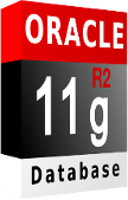
\includegraphics[scale=1]{oracle_11g}} &
              \multicolumn{1}{c}{
\includegraphics[scale=1]{ms_sql}} \\
              \hline
            }
            \tabletail{
              \hline
            }
            \tablelasttail{
              \hline
            }
            \begin{supertabular}{|l|p{5.5cm}|p{5.35cm}|}
              Standarddatumsformat & DD-MON-YY (z. B. 12-NOV-08) & yyyy-mm-ddThh:mm:ss[.mmm] (z. B.  2004-05-23T14:25:10.487) \\
              \hline
              Speicherung & internes numerisches Format & internes numerisches Format \\
              \hline
              Wertebereich & Von 4713 vor Christus bis Dezember 9999. & Zwischen dem 1. Januar 1753 und dem 31. Dezember 9999. \\
              \hline
              Systemdatum anzeigen & SYSDATE / SYSTIMESTAMP & getdate() \\
            \end{supertabular}
          \end{small}
        \end{center}
      \subsection{Datumsarithmetik in Oracle}
        Unter dem Begriff \enquote{Datumsarithmetik} versteht man das Rechnen mit Datumswerten. In Oracle gibt es zwei Möglichkeiten:
        \begin{itemize}
          \item Addition oder Subtraktion von Zahlen zu einem Datumswert
          \item Verwendung von Interval-Literalen
        \end{itemize}
        Führt man Datumsarithmetik durch Addition oder Subtraktion von Zahlen durch gelten folgende Regeln:
        \begin{itemize}
          \item Ganze Zahlen sind Tage, z. B. 1 ist ein Tag, 15 sind fünfzehn Tage
          \item Fraktale (Nachkommastellen) sind Stunden, Minuten und Sekunden, z. B. $\frac{1}{24}=0,041666$ ist eine Stunde oder $\frac{\frac{1}{24}}{60}=0,000694444$ ist eine Minute
          \item Es darf nur addiert oder subtrahiert werden, alle anderen Rechenoperationen sind verboten.
        \end{itemize}
        Einige Beispiele hierzu: So oder in Kommandozeile SQLPLUS !
      
        \begin{lstlisting}[language=oracle_sql,caption={Einfache Datumsarithmetik in Oracle},label=sql03_19]
SELECT to_char (SYSDATE,'DD.MM.yyyyhh24:mm:ss) AS "Datum/Uhrzeit", SYSDATE + 2 AS "2 Tage",
       to_char (SYSDATE - 3 / 24,'DD.MM.yyyyhh24:mm:ss) AS "3 Stunden"
FROM   dual;
        \end{lstlisting}
        \begin{center}
          \begin{small}
            \changefont{pcr}{m}{n}
            \tablefirsthead {
              \multicolumn{1}{l}{\textbf{Datum/Uhrzeit}} &
              \multicolumn{1}{l}{\textbf{2 Tage}} &
              \multicolumn{1}{l}{\textbf{3 Stunden}} \\
              \cmidrule(l){1-1}\cmidrule(l){2-2}\cmidrule(l){3-3}
            }
            \tablehead{}
            \tabletail {
%               \multicolumn{3}{l}{\textbf{1 Zeile ausgewählt}} \\
            }
            \tablelasttail {
              \multicolumn{3}{l}{\textbf{1 Zeile ausgewählt}} \\
            }
            \begin{oraclesql}
              \begin{supertabular}{lll}
                30.04.2013 14:36:24 & 02.05.2013 14:36:24 & 30.04.2013 11:36:24 \\
              \end{supertabular}
            \end{oraclesql}
          \end{small}
        \end{center}
        \subsubsection{Intervall-Literale (Oracle)}
          Intervall-Literale sind dazu da, um Zeiträume anzugeben. Diese
          können in Form von Jahren, Monaten, Tagen, Stunden, Minuten oder
          Sekunden ausgedrückt werden. Es gibt zwei grundsätzlich 
          unterschiedliche Arten von Intervallen:
          \begin{itemize}
            \item YEAR TO MONTH
            \item DAY TO SECOND
          \end{itemize}
          Das YEAR TO MONTH Intervall kann aus bis zu zwei Feldern bestehen,
           wobei das erste die Jahre und das zweite die Monate angibt.
           \tabelle{yeartomonth} zeigt hierzu einige Beispiele.
          \begin{center}
            \tablecaption{Das YEAR TO MONTH Intervall}
            \label{yeartomonth}
            \begin{small}
              \tablefirsthead{
                \multicolumn{1}{c}{\textbf{Beispiel}} &
                \multicolumn{1}{c}{\textbf{Bedeutung}} \\
                \hline
              }
              \tabletail{
                \hline
              }
              \tablelasttail{
                \hline
              }
              \begin{supertabular}{|l|p{9cm}|}
                \texttt{INTERVAL '10' YEAR} & Ein Intervall von 10 Jahren (und 0 Monaten) \\
                \hline
                \texttt{INTERVAL '101' YEAR(3)} & Ein Intervall von 101 Jahren \\
                \hline
                \texttt{INTERVAL '10' YEAR TO YEAR} & Das gleiche wie \texttt{INTERVAL '10' YEAR} \\
                \hline
                \texttt{INTERVAL '10-3' YEAR TO MONTH} & Ein Intervall von 10 Jahren und 3 Monaten \\
                \hline
                \texttt{INTERVAL '27' MONTH} & Ein Intervall von 27 Monaten \\
              \end{supertabular}
            \end{small}
          \end{center}
           Bei der Angabe von Intervall-Literalen gibt es wichtige Dinge zu
           beachten:
          \begin{itemize}
            \item Die Zeitangabe wird immer in Hochkommas gesetzt,
            \item zu jedem Intervall muss angegeben werden, ob es sich um Jahre (YEAR) oder Monate (MONTH) handelt,
            \item die Standardpräzision eines YEAR TO MONTH Intervalls ist immer 2-stellig. Bei drei- oder mehrstelligen Jahresangaben, muss die Präzision angegeben werden. In \beispiel{sql03_20} wird dieses Problem gezeigt.
          \end{itemize}
          \begin{lstlisting}[language=oracle_sql,caption={Richtiger Umgang mit YEAR TO MONTH Intervallen},label=sql03_20]
SELECT SYSDATE - INTERVAL '101' YEAR
FROM   dual;

ORA-01873: the leading precision of the interval is too small 
01873. 00000 -  "the leading precision of the interval is too small"
*Cause:    The leading precision of the interval is too small to store the
           specified interval.
*Action:   Increase the leading precision of the interval or specify an
           interval with a smaller leading precision.

SELECT SYSDATE - INTERVAL '101' YEAR(3)
FROM   dual;
          \end{lstlisting}
\clearpage
          \begin{center}
            \begin{small}
              \changefont{pcr}{m}{n}
              \tablefirsthead {
                \multicolumn{1}{l}{\textbf{SYSDATE-INTERVAL'101(3)'YEAR}} \\
                \cmidrule(l){1-1}
              }
              \tablehead{}
              \tabletail {
                \multicolumn{1}{l}{\textbf{1 Zeile ausgewählt}} \\
              }
              \tablelasttail {
                \multicolumn{1}{l}{\textbf{1 Zeile ausgewählt}} \\
              }
              \begin{oraclesql}
                \begin{supertabular}{l}
                  02.05.03 \\
                \end{supertabular}
              \end{oraclesql}
            \end{small}
          \end{center}
          \begin{merke}
            Mit der Präzision wird angegeben, wie viele Stellen die
            Jahresangabe haben darf. Der Standardwert ist 2.
          \end{merke}
          \beispiel{sql03_20} zeigt, dass die Angaben \languageorasql{INTERVAL
          '101' YEAR} mit dem Oracle-Fehler ORA-01873 scheitert, da die
          Standardpräzision nur 2-stellig ist und daher bei einer
          dreistelligen Jahresangabe die Präzision durch die Angaben
          \languageorasql{YEAR(3)} auf drei Stellen erhöht werden muss.

          Bei der zweiten Art von Intervall-Literal, dem DAY TO SECOND Intervall
          verhält es sich mit der Syntax genauso, wie beim YEAR TO MONTH
          Intervall. \tabelle{daytosecond} zeigt Beispiele für solche
          Intervalle.
          \begin{center}
            \tablecaption{Das DAY TO SECOND Intervall}
            \label{daytosecond}
            \begin{small}
              \tablefirsthead{
                \multicolumn{1}{c}{\textbf{Beispiel}} &
                \multicolumn{1}{c}{\textbf{Bedeutung}} \\
                \hline
              }
              \tabletail{
                \hline
              }
              \tablelasttail{
                \hline
              }
              \begin{supertabular}{|l|p{8.8cm}|}
                \texttt{INTERVAL '8' DAY} & Ein Intervall von 8 Tagen \\
                \hline
                \texttt{INTERVAL '8 4' DAY TO HOUR} & Ein Intervall von 8 Tagen und 4 Stunden \\
                \hline
                \texttt{INTERVAL '8 4:25' DAY TO MINUTE} & Ein Intervall von 8 Tagen, 4 Stunden und 25 Minuten \\
                \hline
                \texttt{INTERVAL '8 4:25:10' DAY TO SECOND} & 8 Tage, 4 Stunden, 25 Minuten und 10 Sekunden \\
                \hline
                \texttt{INTERVAL '120' DAY(3)} & 120 Tage (Präzision 3!!!) \\
                \hline
                \texttt{INTERVAL '3' HOUR} & 3 Stunden \\
                \hline
                \texttt{INTERVAL '3:18' HOUR TO MINUTE} & 3 Stunden und 18 Minuten \\
                \hline
                \texttt{INTERVAL '3:18:10' HOUR TO SECOND} & 3 Stunden, 18 Minuten und 10 Sekunden \\
                \hline
                \texttt{INTERVAL '210' HOUR} & 210 Stunden \\
                \hline
                \texttt{INTERVAL '18' MINUTE} & 18 Minuten \\
                \hline
                \texttt{INTERVAL '18:10' MINUTE TO SECOND} & 18 Minuten und 10 Sekunden \\
                \hline
                \texttt{INTERVAL '120' MINUTE} & 120 Minuten \\
                \hline
                \texttt{INTERVAL '10' SECOND} & 10 Sekunden \\
                \hline
                \texttt{INTERVAL '180' SECOND} & 180 Sekunden \\
              \end{supertabular}
            \end{small}
          \end{center}
          \begin{merke}
            Für das DAY TO SECOND Intervall gelten, bezüglich der
            Präzision, die gleichen Regeln, wie beim YEAR TO MONTH Intervall.
          \end{merke}
          Manchmal ist es notwendig Zeitintervalle zu formulieren, die zu keinem
          der beiden Typen passen. Dies könnte z. B. 4 Jahre, 10 Monate, 8
          Tage und 5 Stunden sein. Auch das ist möglich, wie
          \beispiel{sql03_21} zeigt.
\clearpage
          \begin{lstlisting}[language=oracle_sql,caption={Ein komplexe Zeitintervall},label=sql03_21]
SELECT SYSDATE - INTERVAL '4-10' YEAR TO MONTH -
       INTERVAL '8 5' DAY TO HOUR AS Interval
FROM   dual;
          \end{lstlisting}
          \begin{center}
            \begin{small}
              \changefont{pcr}{m}{n}
              \tablefirsthead {
                \multicolumn{1}{l}{\textbf{INTERVAL}} \\
                \cmidrule(l){1-1}
              }
              \tablehead{}
              \tabletail {
                \multicolumn{1}{l}{\textbf{1 Zeile ausgewählt}} \\
              }
              \tablelasttail {
                \multicolumn{1}{l}{\textbf{1 Zeile ausgewählt}} \\
              }
              \begin{oraclesql}
                \begin{supertabular}{l}
                  24.06.08 \\
                \end{supertabular}
              \end{oraclesql}
            \end{small}
          \end{center}
      \subsection{Datumsarithmetik in MS SQL Server}
        Unter dem Begriff \enquote{Datumsarithmetik} versteht man das Rechnen mit Datumswerten. In SQL Server stehen hierfür die Funktionen:
        \begin{itemize}
          \item \languagemssql{DATEADD}
          \item \languagemssql{DATEDIFF}
          \item \languagemssql{DATEPART}
          \item \languagemssql{DATENAME}
        \end{itemize}
        zur Verfügung. Sie verarbeiten Datumswerte und Zeitintervalle.

        \begin{merke}
          Die verschiedenen Intervalle, die für die genannten Funktionen zur
          Verfügung stehen sind: \identifier{NANOSECOND},
          \identifier{MICROSECOND},  \identifier{MILLISECOND},
          \identifier{SECOND}, \identifier{MINUTE}, \identifier{HOUR},
          \identifier{WEEKDAY}, \identifier{WEEK}, \identifier{DAY},
          \identifier{DAYOFYEAR}, \identifier{MONTH}, \identifier{QUARTER},
          \identifier{YEAR}.
        \end{merke}
        \subsubsection{Die Funktion DATEADD - Datumswerte addieren}
          \beispiel{sql03_22} zeigt, die Anwendung der Funktion \languagemssql{DATEADD}
          \begin{lstlisting}[language=ms_sql,caption={Die Funktion \languagemssql{DATEADD} in SQL Server},label=sql03_22]
SELECT GETDATE(), DATEADD(DAY, 1, GETDATE()), DATEADD(HOUR, 1, GETDATE())
       DATEADD(MINUTE, 1, GETDATE());
          \end{lstlisting}
          \begin{center}
            \begin{small}
              \changefont{pcr}{m}{n}
              \tablefirsthead{
                \multicolumn{1}{l}{\textbf{(Kein Spaltenname)}} &
                \multicolumn{1}{l}{\textbf{(Kein Spaltenname)}} \\
                \cmidrule(l){1-1}\cmidrule(l){2-2}
              }
              \tabletail{}
              \tablelasttail{}
              \begin{mssql}
                \begin{supertabular}{ll}
                  2013-05-02 12:00:36.047 & 2013-05-03 12:00:36.047 \\
                  \textbf{(Kein Spaltenname)} & \textbf{(Kein Spaltenname)} \\
                  \cmidrule(l){1-1}\cmidrule(l){2-2}
                  2013-05-02 13:00:36.047 & 2013-05-02 12:01:36.050 \\
                \end{supertabular}
              \end{mssql}
            \end{small}
          \end{center}
          Diese Funktion ermöglicht es, ein Zeitintervall zu einem Datum zu addieren.
        \subsubsection{Die Funktion DATEDIFF - Eine Differenz bilden}
          Um die Möglichkeit zu schaffen, die Differenz zwischen zwei Datumswerten zu bilden, wurde die Funktion \languagemssql{DATEDIFF} in MS SQL Server integriert.
          \begin{lstlisting}[language=ms_sql,caption={Die Funktion \languagemssql{DATEDIFF} in SQL Server},label=sql03_23]
SELECT GETDATE(),
       DATEDIFF(DAY, CONVERT(DATETIME2, '01.05.2010', 104), GETDATE()),
       DATEDIFF(YEAR, CONVERT(DATETIME2, '01.05.2010', 104), GETDATE());
          \end{lstlisting}
          \begin{center}
            \begin{small}
              \changefont{pcr}{m}{n}
              \tablefirsthead{
                \multicolumn{1}{l}{\textbf{(Kein Spaltenname)}} &
                \multicolumn{1}{l}{\textbf{(Kein Spaltenname)}} &
                \multicolumn{1}{l}{\textbf{(Kein Spaltenname)}} \\
                \cmidrule(l){1-1}\cmidrule(l){2-2}\cmidrule(l){3-3}
              }
              \tabletail{}
              \tablelasttail{}
              \begin{mssql}
                \begin{supertabular}{lll}
                  2013-05-13 11:49:34.730 & 1108 & 3 \\
                \end{supertabular}
              \end{mssql}
            \end{small}
          \end{center}
          Das Ergebnis dieser Funktion ist die Differenz zwischen dem Startdatum und dem Enddatum, in dem angegebenen Intervall.
        \subsubsection{Die Funktionen DATEPART/DATENAME - Teile eines Datums extrahieren}
          Mit Hilfe der Funktionen \languagemssql{DATEPART} und \languagemssql{DATENAME} können Teile eines Datums, als Zeichenkette extrahiert werden.
          \begin{lstlisting}[language=ms_sql,caption={\languagemssql{DATEPART} und \languagemssql{DATENAME} in SQL Server},label=sql03_24]
SELECT GETDATE(), DATEPART(YEAR, GETDATE()),
       DATEPART(MONTH, GETDATE()) AS "DATEPART",
       DATENAME(MONTH, GETDATE()) AS "DATENAME";
          \end{lstlisting}
          \begin{center}
            \begin{small}
              \changefont{pcr}{m}{n}
              \tablefirsthead{
                \multicolumn{1}{l}{\textbf{(Kein Spaltenname)}} &
                \multicolumn{1}{l}{\textbf{(Kein Spaltenname)}} \\
                \cmidrule(l){1-1}\cmidrule(l){2-2}
              }
              \tabletail{}
              \tablelasttail{}
              \begin{mssql}
                \begin{supertabular}{ll}
                  2013-05-13 11:49:34.730 & 2013 \\
                  \textbf{(DATEPART)} & \textbf{(DATENAME)} \\
                  \cmidrule(l){1-1}\cmidrule(l){2-2}
                  5 & Mai \\
                \end{supertabular}
              \end{mssql}
            \end{small}
          \end{center}
    \section{Sonstige Funktionen}
      Das NULL-Werte etwas besonderes darstellen wurde in \abschnitt{nullvalues}
      bereits erläutert. Welche Effekte durch diese Besonderheit auftreten,
      war in \beispiel{sql01_06} zu sehen. Dieser Abschnitt zeigt nun, wie man
      mit der Besonderheit der NULL-Werte umgeht.

      Oracle und SQL Server kennen Funktionen, um dieser Problematik Herr zu
      werden. In Oracle ist es die \languageorasql{NVL}, in SQL Server die
      \languagemssql{ISNULL} (nicht zu verwechseln mit \languagemssql{IS NULL})
      Funktion. Beide Funktionen ersetzen NULL-Werte durch einen nahezu
      freiwählbaren Ersatzwert. \beispiel{sql03_25} zeigt die Funktion
      \languageorasql{NVL} in Oracle.
      \begin{lstlisting}[language=oracle_sql,caption={Die Funktion \languageorasql{NVL}},label=sql03_25]
SELECT Gehalt + (Gehalt / 100 * Provision) AS "Mit NULL",
       Gehalt + (Gehalt / 100 * NVL(Provision, 0)) AS "Ohne NULL"
FROM   Mitarbeiter;
      \end{lstlisting}
      \begin{center}
        \begin{small}
          \changefont{pcr}{m}{n}
          \tablefirsthead {
            \multicolumn{1}{r}{\textbf{Mit NULL}} &
            \multicolumn{1}{r}{\textbf{Ohne NULL}} \\
            \cmidrule(r){1-1}\cmidrule(r){2-2}
          }
          \tablehead{}
          \tabletail {
            \multicolumn{2}{l}{\textbf{101 Zeilen ausgewählt}} \\
          }
          \tablelasttail {
            \multicolumn{2}{l}{\textbf{101 Zeilen ausgewählt}} \\
          }
          \begin{oraclesql}
            \begin{supertabular}{rr}
              & 30000 \\
              & 30000 \\
              \dots & \dots \\
              2400 & 2400 \\
              2500 & 2500 \\
              & 2000 \\
              & 1500 \\
              1200 & 1200 \\
            \end{supertabular}
          \end{oraclesql}
        \end{small}
      \end{center}
      \begin{merke}
        In \beispiel{sql03_24} geschieht folgendes:
        \begin{itemize}
          \item Bei der Berechnung von \textit{Gehalt + (Gehalt / 100 * Provision)} kommt die Problematik mit den NULL-Werten zum Tragen und es wird, in einigen Zeilen, der Wert NULL angezeigt.
          \item Bei der Berechnung von \textit{Gehalt + (Gehalt / 100 * NVL(Provision, 0))} werden die in der Spalte \identifier{Provision} auftretenden NULL-Werte von NVL durch den Wert 0 ersetzt, so dass die Berechnung ein gültiges Ergebnis liefern kann.
        \end{itemize}
      \end{merke}
      Gleiches geschieht beim MS SQL Server durch die Funktion \languagemssql{ISNULL}, wie in \beispiel{sql03_26} zu sehen ist.
      \begin{lstlisting}[language=ms_sql,caption={Die Funktion \languageorasql{ISNULL}},label=sql03_26]
SELECT Gehalt + (Gehalt / 100 * Provision) AS "Mit NULL",
       Gehalt + (Gehalt / 100 * ISNULL(Provision, 0)) AS "Ohne NULL"
FROM   Mitarbeiter;
      \end{lstlisting}
\clearpage
      \begin{center}
        \begin{small}
          \changefont{pcr}{m}{n}
          \tablefirsthead {
            \multicolumn{1}{l}{\textbf{Mit NULL}} &
            \multicolumn{1}{l}{\textbf{Ohne NULL}} \\
            \cmidrule(l){1-1}\cmidrule(l){2-2}
          }
          \tablehead{}
          \tabletail {
            \multicolumn{2}{l}{\textbf{101 Zeilen ausgewählt}} \\
          }
          \tablelasttail {
            \multicolumn{2}{l}{\textbf{101 Zeilen ausgewählt}} \\
          }
          \begin{mssql}
            \begin{supertabular}{ll}
              & 30000.000000 \\
              & 30000.000000 \\
              \dots & \dots \\
              2400.000000 & 2400.000000 \\
              2500.000000 & 2500.000000 \\
            \end{supertabular}
          \end{mssql}
        \end{small}
      \end{center}
    \section{Datentypen}
      Datentypen helfen in der Programmierung konkrete Wertebereiche und darauf
      definierte Operationen festzulegen. Ist eine Tabellenspalte beispielsweise
      so erstellt worden, dass sie nur Datumswerte akzeptiert, können dort
      keine anderen Werte, wie z. B. Zahlen oder Zeichenketten, gespeichert
      werden. Auch die für Datumswerte definierten Operationen sind exakt
      begrenzt. Während Addition oder Subtraktion von Zahlen zu einem
      Datumswert erlaubt sind, ist die Addition zweier Datumswerte nicht
      möglich. Ebenso verhält es sich mit Zahlen und Zeichenketten. Auf
      Zahlen können die Rechenoperationen der Arithmetik (+, -, * und /)
      angewandt werden, auf Zeichenketten nicht.

      \tabelle{datatypes} liefert einen kleinen Ausschnitt aus der Menge der
      Datentypen, die Oracle und SQL Server kennen und erläutert deren
      Bedeutung.
      \begin{center}
        \tablecaption{Datentypen}
        \label{datatypes}
        \begin{small}
          \tablefirsthead{
            \multicolumn{1}{c}{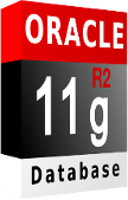
\includegraphics[scale=1]{oracle_11g}} &
            \multicolumn{1}{c}{
\includegraphics[scale=1]{ms_sql}} &
            \multicolumn{1}{c}{\textbf{Bedeutung}} \\
            \hline
          }
          \tabletail{
            \hline
          }
          \tablelasttail{
            \hline
          }
          \begin{supertabular}{|l|l|p{8cm}|}
            \identifier{NUMBER} & \identifier{NUMERIC} & Numerische Datentypen
            mit fester Genauigkeit und fester Anzahl von Dezimalstellen. \\
            \hline
            \identifier{DATE} & \identifier{DATETIME2} & Datums- und
            Zeitdatentypen zum Darstellen von Datum und Tageszeit. \\
            \hline
            \identifier{TIMESTAMP} & \identifier{DATETIME2} & Ein Datums- und
            Zeitdatentyp mit höherer Genauigkeit als \identifier{DATE}. \\
            \hline
            \identifier{VARCHAR2} & \identifier{VARCHAR} &
            Nicht-Unicode-Zeichendaten variabler Länge. \\
            \hline
            \identifier{CHAR} & \identifier{CHAR} & Nicht-Unicode-Zeichendaten
            fester Länge \\
          \end{supertabular}
        \end{small}
      \end{center}
      \subsection{Numerische Datentypen}
        \subsubsection{Aufbau}
          Die beiden Datentypen \identifier{NUMBER} (Oracle) und
          \identifier{NUMERIC} (SQL Server) sind dazu da, um positive oder
          negative numerische Werte, mit oder ohne Nachkommastellen,
          aufzunehmen. Die Wertebereiche, die beide Datentypen aufnehmen
          können, unterscheiden sich.
\clearpage
          \begin{center}
            \tablecaption{Datentypen}
            \label{numericranges}
            \begin{small}
              \tablefirsthead{
                \multicolumn{1}{c}{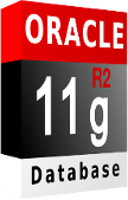
\includegraphics[scale=1]{oracle_11g}} &
                \multicolumn{1}{c}{
\includegraphics[scale=1]{ms_sql}} &
                \multicolumn{1}{c}{\textbf{Wertebereich}} \\
                \hline
              }
              \tabletail{
                \hline
              }
              \begin{supertabular}{|l|l|p{8cm}|}
                \identifier{NUMBER} & & $\pm1.0*10^{-130}$ bis $\pm1.0*10^{126}-1$ \\
                \hline
                & \identifier{NUMERIC} & $-1.0*10^{-38}$ bis $1.0*10^{38}-1$ \\
              \end{supertabular}
            \end{small}
          \end{center}
          \begin{merke}
            Zahlen die größer oder kleiner als die angegebenen
            Wertebereiche sind, können nicht aufgenommen werden.
          \end{merke}
        \subsubsection{Präzision und Skalarität}
          Unter der Präzision versteht man die Angabe, bei wie vielen Stellen
          insgesamt noch ein rundungsfehlerfreies Ergebnis angezeigt werden
          kann. Die maximale Präzision beider Typen beschränkt sich auf
          Zahlen, die kleiner oder gleich $10^{38}$ sind. Daraus folgt, dass
          solange sich eine Zahl in diesem Wertebereich befindet, sie frei von
          Rundungsfehlern ist. Ist sie größer, können Rundungsfehler
          auftreten. Beim Microsoft SQL Server stellt sich diese Problematik
          nicht, da bei \identifier{NUMERIC} der Wertebereich auf $10^{38}$
          beschränkt ist.

          Um die benötigte Präzision einstellen zu können, ist es auf beiden Systemen möglich, die maximale Anzahl Stellen, die eine Tabellenspalte aufnehmen können soll, auf einen Wert zwischen 1 und 38 einzuschränken. Ist eine Spalte, z. B. auf neun Stellen begrenzt, ist die größte Zahl, die in diese Spalte eingefügt werden kann, die 999.999.999.

          Mit Hilfe der Skalarität kann manuell festgelegt werden, wie viele der durch die Präzision angegebenen Stellen rechts vom Komma verwendet werden. Wird eine Spalte mit einer Präzision von neun und einer Skalarität von zwei definiert, kann sie maximal sieben Stellen links und zwei Stellen rechts vom Komma enthalten. Die größte Zahl, die in eine solche Spalte eingefügt werden kann, ist somit die 9.999.999,99.
      \subsection{Zeichendatentypen}
        \subsubsection{Typen fester Länge}
          Bei den Zeichendatentypen wird nach Typen fester Länge und Typen variabler Länge unterschieden. Der Datentyp zur Aufnahme von Zeichenketten fester Länge, heißt in beiden Systemen \identifier{CHAR}. Datentypen fester Länge haben ihren Namen daher, dass bei der Definition einer Tabellenspalte, mit einem solchen Typ, die Länge der Spalte fest angegeben werden muss.

          \begin{merke}
            Der Speicherplatzverbrauch einer solchen Spalte richtet sich nicht nach ihrem Inhalt (Anzahl der enthaltenen Zeichen), sondern nach der vorgegebenen Größe. Wird eine Spalte mit einer Größe von 20 definiert, beträgt ihr Speicherplatzverbrauch 20, 40 oder 80 Byte\footnote{Je nach dem, welcher Zeichensatz verwendet wird, werden pro Zeichen 1, 2 oder 4 Byte Speicherplatz benötigt.}. Dies trifft auch dann zu, wenn die Spalte nur ein einziges Zeichen enthält.
          \end{merke}
        \subsubsection{Typen variabler Länge}
          Die Zeichendatentypen variabler Länge unterscheiden sich in Oracle und SQL Server nur in ihrem Namen. SQL Server verwendet die SQL-92-Standard gemäße Bezeichnung \identifier{VARCHAR}, während Oracle die Bezeichnung \identifier{VARCHAR2}, als Synonym für VARCHAR verwendet. Die Nutzung von \identifier{VARCHAR} ist aber auch in Oracle zulässig.

          \begin{merke}
            Im Unterschied zu den Typen fester Länge, ergibt sich der Speicherplatzverbrauch bei Typen variabler Länge nicht durch eine fest definierte Größe, sondern anhand ihres Inhalts. Es kann eine maximale Größe angegeben werden. Die Spalte kann dann maximal so viele Zeichen aufnehmen, wie angegeben.
          \end{merke}
        \subsection{Datums- und Zeittypen}
          Zur Speicherung von Datums- und Zeitwerten kennt Oracle die beiden Datentypen \identifier{DATE} und \identifier{TIMESTAMP}. Microsoft SQL Server verwendet \identifier{DATETIME2}.

          \begin{merke}
            In MS SQL Server gibt es auch einen Datentyp \identifier{TIMESTAMP}. Dieser ist jedoch, abweichend vom SQL-2003-Standard, nicht zur Speicherung von Datums- und Zeitwerten vorgesehen und seit SQL Server 2008 als veraltet eingestuft.
          \end{merke}
          \subsubsection{Oracle - DATE und TIMESTAMP}
            Der Datentyp \identifier{DATE} speichert seine Datumswerte in einem internen, numerischen Format. Er berücksichtigt dabei: Jahrzehnt, Jahr, Monat, Tag, Stunde, Minute, Sekunde. Der Typ \identifier{TIMESTAMP} ist eine Erweiterung. Er kann Datums- und Zeitangaben auf bis zu 9 Stellen (Nanosekunde) genau, im Sekundenbereich speichern.
          \subsubsection{SQL Server - DATETIME2}
            Werte des \identifier{DATETIME2}-Datentyps werden von der Microsoft SQL Server 2008 R2 Database Engine (Datenbankmodul) intern, als zwei 4 Byte lange, ganze Zahlen, gespeichert. Die ersten 4 Byte enthalten die Anzahl von Tagen, vor oder nach dem Referenzdatum, dem 1. Januar 1900. Die anderen 4 Byte speichern die Tageszeit, die als Anzahl von Millisekunden seit Mitternacht dargestellt wird.
    \section{Konvertierung von Datentypen}
      Unter der Konvertierung von Datentypen versteht man das Umwandeln eines Wertes, eines bestimmten Typs, in einen anderen Typ. Beispielsweise kann eine Zeichenkette \enquote{1234} in die gleichlautende Zahl \enquote{1234} umgewandelt werden. Intern wird nur der Datentyp von VARCHAR/VARCHAR2 auf NUMERIC/NUMBER geändert. Dies ist z. B. notwendig, um arithmetische Operationen durchzuführen.
      \subsection{Implizite Datentypkonvertierung}
        \begin{merke}
				Unter der impliziten Konvertierung versteht man, dass automatische Umwandeln eines Datentyp durch das DBMS in einen Anderen.
        \end{merke}
        In \beispiel{sql03_27} wird die implizite Konvertierung der Gehälter in Zeichenketten gezeigt.
        \begin{lstlisting}[language=oracle_sql,caption={Implizite Konvertierung von \identifier{NUMBER} zu \identifier{VARCHAR2}},label=sql03_27]
SELECT 'Das Gehalt von ' || Nachname || ' betraegt: ' || gehalt
       AS "Implizite Konvertierung"
FROM   Mitarbeiter;
        \end{lstlisting}
        \begin{center}
          \begin{small}
            \changefont{pcr}{m}{n}
            \tablefirsthead {
              \multicolumn{1}{l}{\textbf{Implizite Konvertierung}} \\
              \cmidrule(l){1-1}
            }
            \tablehead{}
            \tabletail {
              \multicolumn{1}{l}{\textbf{101 Zeilen ausgewählt}} \\
            }
            \tablelasttail {
              \multicolumn{1}{l}{\textbf{101 Zeilen ausgewählt}} \\
            }
            \begin{oraclesql}
              \begin{supertabular}{l}
                Das Gehalt von Winter betraegt: 88000 \\
                Das Gehalt von Werner betraegt: 50000 \\
                Das Gehalt von Seifert betraegt: 50000 \\
                Das Gehalt von Schwarz betraegt: 30000 \\
              \end{supertabular}
            \end{oraclesql}
          \end{small}
        \end{center}
\clearpage
        Damit Oracle eine Ausgabe wie \enquote{Das Gehalt von Winter betraegt:
        88000} darstellen kann, muss ein einheitlicher Datentyp geschaffen
        werden. Hierzu wird ein Ausdruck in zwei Teile zerlegt, einen linken und
        einen rechten. Der rechte Teil wird dann, sofern möglich, in den
        Datentyp des Linken konvertiert. Für \beispiel{sql03_27} bedeutet dies
        konkret:
        \begin{itemize}
          \item Linke Seite: \languageorasql{'Das Gehalt von ' || Nachname || ' betraegt: '}
          \item Rechte Seite: \languageorasql{Gehalt}
          \item Datentyp der linken Seite: \identifier{VARCHAR2}
          \item Datentyp der rechten Seite: \identifier{NUMBER}
          \item Daraus folgt: Konvertiere \identifier{NUMBER} nach \identifier{VARCHAR2}
        \end{itemize}
        Nicht immer ist das Konvertieren eines Datentyps in einen anderen möglich. Für die implizite Konvertierung gibt es einige Einschränkungen.
        \begin{itemize}
          \item Der Wert selbst muss in den neuen Typ konvertierbar sein. Beispielsweise kann die Zeichenkette ABCDE nicht in eine Zahl oder ein Datum umgewandelt werden, da sie kein sinnvolles Datum darstellt.
          \item Der Datentyp selbst muss in den neuen Datentyp konvertierbar sein. Zum Beispiel kann Oracle einen Wert des Datentyps NUMBER nicht direkt in einen Wert des Typs DATE konvertieren, da hierzu ein Referenzdatum benötigt wird.
        \end{itemize}
        Die beiden folgenden Tabellen zeigen, welche impliziten Typkonvertierung in Oracle und SQL Server möglich sind. Dabei wird immer zugrunde gelegt, dass der betreffende Wert auch konvertierbar ist.
        \begin{center}
          \tablecaption{Implizite Datentypkonvertierung in Oracle}
          \label{oracleimplicit}
          \begin{small}
            \tablefirsthead{
              \multicolumn{6}{c}{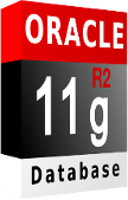
\includegraphics[scale=1]{oracle_11g}} \\
              \multicolumn{1}{c}{} &
              \multicolumn{1}{c}{\textbf{NUMBER}} &
              \multicolumn{1}{c}{\textbf{VARCHAR2}} &
              \multicolumn{1}{c}{\textbf{CHAR}} &
              \multicolumn{1}{c}{\textbf{DATE}} &
              \multicolumn{1}{c}{\textbf{TIMESTAMP}} \\
              \hline
            }
            \tabletail{
              \hline
            }
            \tablelasttail{
              \hline
            }
            \begin{supertabular}{|l|c|c|c|c|c|}
              NUMBER    & -- & X  & X  & -- & -- \\
              \hline
              VARCHAR2  & X  & -- & X  & X  & X \\
              \hline
              CHAR      & X  & X  & -- & X  & X \\
              \hline
              DATE      & -- & X  & X  & -- & -- \\
              \hline
              TIMESTAMP & X  & X  & X  & -- & -- \\
            \end{supertabular}
          \end{small}
        \end{center}
\clearpage
        \begin{center}
          \tablecaption{Implizite Datentypkonvertierung in Microsoft SQL Server}
          \label{mssqlimplicit}
          \begin{small}
            \tablefirsthead{
              \multicolumn{5}{c}{
\includegraphics[scale=1]{ms_sql}} \\
              \multicolumn{1}{c}{} &
              \multicolumn{1}{c}{\textbf{NUMERIC}} &
              \multicolumn{1}{c}{\textbf{VARCHAR}} &
              \multicolumn{1}{c}{\textbf{CHAR}} &
              \multicolumn{1}{c}{\textbf{DATETIME2}} \\
              \hline
            }
            \tabletail{
              \hline
            }
            \tablelasttail{
              \hline
            }
            \begin{supertabular}{|l|c|c|c|c|}
              NUMERIC   & -- & X  & X  & X \\
              \hline
              VARCHAR   & X  & -- & X  & X \\
              \hline
              CHAR      & X  & X  & -- & X \\
              \hline
              DATETIME  & -- & X  & X  & -- \\
            \end{supertabular}
          \end{small}
        \end{center}
        \begin{merke}
            Der SQL Server besitzt intern eine Rangfolge seiner Datentypen. Dadurch wird bei der impliziten Konvertierung der Datentyp mit der niedrigeren Rangfolge in den Datentyp mit der höheren Rangfolge umgewandelt.
        \end{merke}
        \begin{literaturinternet}
          \item \cite{autoId8}
          \item \cite{ms191530}
          \item \cite{ms190309}
        \end{literaturinternet}
      \subsection{Explizite Datentypkonvertierung}
        \subsubsection{Explizite Datentypkonvertierung in Oracle}
          \begin{merke}
            Bei der expliziten Datentypkonvertierung werden Werte, mit Hilfe von
            Funktionen, von einem Datentyp in einen anderen konvertiert.
          \end{merke}
          Oracle kennt für das explizite Konvertieren von Daten verschiedene
          Funktionen. Diese sind:
          \begin{itemize}
            \item \languageorasql{TO\_CHAR}
            \item \languageorasql{TO\_DATE}
            \item \languageorasql{TO\_TIMESTAMP}
            \item \languageorasql{TO\_NUMBER}
          \end{itemize}
          Es existieren noch weitere Funktionen, die an dieser Stelle jedoch
          ungenannt bleiben. Die folgende Tabelle zeigt eine Übersicht, welche
          Datentypen, mit Hilfe der expliziten Datentypkonvertierung umgewandelt
          werden können.
          \begin{center}
            \tablecaption{Explizite Datentypkonvertierung in Oracle}
            \label{oracleexplicit}
            \begin{small}
              \tablefirsthead{
                \multicolumn{6}{c}{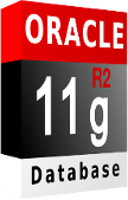
\includegraphics[scale=1]{oracle_11g}} \\
                \multicolumn{1}{c}{} &
                \multicolumn{1}{c}{\textbf{NUMBER}} &
                \multicolumn{1}{c}{\textbf{VARCHAR2}} &
                \multicolumn{1}{c}{\textbf{CHAR}} &
                \multicolumn{1}{c}{\textbf{DATE}} &
                \multicolumn{1}{c}{\textbf{TIMESTAMP}} \\
                \hline
              }
              \tabletail{
                \hline
              }
              \begin{supertabular}{|l|c|c|c|c|c|}
                NUMBER    & -- & TO\_CHAR & TO\_CHAR            &          & -- \\
                \hline
                VARCHAR2  & TO\_NUMBER    & --       & --       & TO\_DATE & TO\_TIMESTAMP \\
                \hline
                CHAR      & TO\_NUMBER    & --       & --       & TO\_DATE & TO\_TIMESTAMP \\
                \hline
                DATE      & --            & TO\_CHAR & TO\_CHAR & --       & TO\_TIMESTAMP \\
                \hline
                TIMESTAMP & --            & TO\_CHAR & TO\_CHAR & --       & -- \\
              \end{supertabular}
            \end{small}
          \end{center}
          \beispiel{sql03_28} zeigt die Umwandlung des Systemdatums in eine
          Zeichenkette.
          \begin{lstlisting}[language=oracle_sql,caption={Explizite Datentypkonvertierung in Oracle},label=sql03_28]
SELECT TO_CHAR(SYSDATE)
FROM   dual;
          \end{lstlisting}
          \begin{center}
            \begin{small}
              \changefont{pcr}{m}{n}
              \tablefirsthead {
                \multicolumn{1}{l}{\textbf{TO\_CHAR(SYSDATE)}} \\
                \cmidrule(l){1-1}
              }
              \tablehead{}
              \tabletail {
%                 \multicolumn{1}{l}{\textbf{1 Zeile ausgewählt}} \\
              }
              \tablelasttail {
                \multicolumn{1}{l}{\textbf{1 Zeile ausgewählt}} \\
              }
              \begin{oraclesql}
                \begin{supertabular}{l}
                  02.05.13 \\
                \end{supertabular}
              \end{oraclesql}
            \end{small}
          \end{center}
          Tatsächlich geschieht in \beispiel{sql03_28} nichts sichtbares,
          dennoch hat eine Umwandlung stattgefunden. Um diese sichtbar zu
          machen, kann während der Konvertierung eine Formatierung des
          Ergebniswertes durchgeführt werden.
          \begin{lstlisting}[language=oracle_sql,caption={Konvertierung und Formatierung},label=sql03_29]
SELECT TO_CHAR(SYSDATE, 'DD.MM.YYYY')
FROM   dual;
          \end{lstlisting}
          \begin{center}
            \begin{small}
              \changefont{pcr}{m}{n}
              \tablefirsthead {
                \multicolumn{1}{l}{\textbf{TO\_CHAR(SYSDATE,'DD.MM.YYYY')}} \\
                \cmidrule(l){1-1}
              }
              \tablehead{}
              \tabletail {
                \multicolumn{1}{l}{\textbf{1 Zeile ausgewählt}} \\
              }
              \tablelasttail {
                \multicolumn{1}{l}{\textbf{1 Zeile ausgewählt}} \\
              }
              \begin{oraclesql}
                \begin{supertabular}{l}
                  02.05.2013 \\
                \end{supertabular}
              \end{oraclesql}
            \end{small}
          \end{center}
          Das zweite Argument der \languageorasql{TO\_CHAR}-Funktion, \languageorasql{'DD.MM.YYYY'}, wird als \enquote{Formatmodell} bezeichnet. Mit Hilfe dieser Buchstabenkombination wird das Ausgabeformat für die Zeichenfolge festgelegt. Die Bedeutung der Buchstaben ist:
          \begin{itemize}
            \item \languageorasql{DD}: Tag 2-stellig
            \item \languageorasql{MM}: Monat 2-stellig
            \item \languageorasql{YYYY}: Jahr 4-stellig
          \end{itemize}
          \beispiel{sql03_30} zeigt ein weiteres, individuelles Formatmodell für einen Datumswert.
          \begin{lstlisting}[language=oracle_sql,caption={Ein anderes Formatmodell},label=sql03_30]
SELECT TO_CHAR(SYSDATE, 'DD. MON YYYY')
FROM   dual;
          \end{lstlisting}
          \begin{center}
            \begin{small}
              \changefont{pcr}{m}{n}
              \tablefirsthead {
                \multicolumn{1}{l}{\textbf{TO\_CHAR(SYSDATE,'DD.MONYYYY')}} \\
                \cmidrule(l){1-1}
              }
              \tablehead{}
              \tabletail {
                \multicolumn{1}{l}{\textbf{1 Zeile ausgewählt}} \\
              }
              \tablelasttail {
                \multicolumn{1}{l}{\textbf{1 Zeile ausgewählt}} \\
              }

              \begin{oraclesql}
                \begin{supertabular}{l}
                  02. MAI 2013 \\
                \end{supertabular}
              \end{oraclesql}
            \end{small}
          \end{center}
          Die Buchstabenkombination \languageorasql{MON} sorgt dafür, dass der Monat als Wort angezeigt wird. Ob \enquote{Mai} oder \enquote{May} angezeigt wird, ist abhängig von den Ländereinstellungen der Datenbank.

          \begin{merke}
            Ein Formatmodell ist eine Zeichenfolge, die das Format eines Datums oder eines numerischen Wertes beschreibt. Ein Formatmodell ändert nicht die interne Darstellung eines Wertes in der Datenbank, sondern formatiert lediglich die Ausgabe. Es setzt sich aus mehreren Formatelemten zusammen, z. B. DD oder MM oder YYYY.
          \end{merke}
          Welche Formatmodelle erstellt werden können, hängt davon ab, welche Formatelemte die einzelnen Funktionen kennen. Die folgenden Literaturhinweise führen zu den Tabellen in der Oracle Online-Dokumentation, die alle existierenden Formatelemente enthält.
          \begin{literaturinternet}
            \item \cite{i34570}
            \item \cite{i34924}
          \end{literaturinternet}

          \begin{merke}
            Für die Funktion \languageorasql{TO\_CHAR} existiert keine eigenständige Zusammenstellung von Formatelementen, da sie sowohl Datumswerte in Text, als auch Zahlen in Text konvertiert und dafür die Formatelemente von \languageorasql{TO\_NUMBER} und \languageorasql{TO\_DATE} nutzt.
          \end{merke}
        \subsubsection{Explizite Datentypkonvertierung in Microsoft SQL Server}
          \begin{merke}
            Bei der expliziten Datentypkonvertierung werden Werte, mit Hilfe von Funktionen, von einem Datentyp in einen anderen konvertiert.
          \end{merke}
          MS SQL Server kennt die Funktion \languagemssql{CONVERT} zur Konvertierung von Datentypen \footnote{Es gibt zusätzlich die Funktion CAST. Jedoch wird seitens Microsoft empfohlen, \languagemssql{CONVERT} zu nutzen, obgleich die Verwendung von CAST dem ISO-Standard entsprechen würde.}. Die Syntax dieser Funktion lautet:
          \begin{lstlisting}[language=ms_sql,caption={Die Syntax der CONVERT-Funktion in MS SQL Server},label=sql03_31]
CONVERT( <Datentyp>[(Laenge)], <Ausdruck>[, Style])
          \end{lstlisting}
          \begin{center}
            \tablecaption{Funktionsargumente von CONVERT}
            \label{argconvert}
            \begin{small}
              \tablefirsthead{
                \multicolumn{1}{c}{\textbf{Argument}} &
                \multicolumn{1}{c}{\textbf{Beispiel}} &
                \multicolumn{1}{c}{\textbf{Erläuterung}} \\
                \hline
              }
              \tabletail{
                \hline
              }
              \tablelasttail{
                \hline
              }
              \begin{supertabular}{|l|c|p{8.5cm}|}
                \textless Datentyp\textgreater & DATETIME & Dies ist die Angabe des Datentyps, in den \textless Ausdruck\textgreater\ konvertiert werden soll.  Für jeden Datentyp kann optional eine Länge mit angegeben werden.\\
                \hline
                \textless Ausdruck\textgreater & '16.01.2009'& <Ausdruck> ist eine Zeichenkette, Zahl, ein Datums- Zeitwert oder eine Funktion. \\
                \hline
                [Style] & 104 & Optional kann bei der CONVERT-Funktion ein Formatmodell angegeben werden. \\
              \end{supertabular}
            \end{small}
          \end{center}
          Ein Formatmodell legt fest, wie ein Eingabewert interpretiert oder ein Ausgabewert formatiert werden soll. Alle Formatmodelle sind durch Zahlen kodiert.

          Die Bedeutung der Formatmodelle soll konkret anhand von \beispiel{sql03_32} erläutert werden.
          \begin{lstlisting}[language=ms_sql,caption={CONVERT mit Formatmodell},label=sql03_32]
SELECT CONVERT(DATETIME2, '02.05.2013', 104)
          \end{lstlisting}
          \begin{center}
            \begin{small}
              \changefont{pcr}{m}{n}
              \tablefirsthead{
                \multicolumn{1}{l}{\textbf{(Kein Spaltenname)}} \\
                \cmidrule(l){1-1}
              }
              \tabletail{}
              \tablelasttail{}
              \begin{mssql}
                \begin{supertabular}{l}
                  2013-05-02 00:00:00.0000000 \\
                \end{supertabular}
              \end{mssql}
            \end{small}
          \end{center}
          \beispiel{sql03_32} zeigt die Konvertierung der Zeichenkette \enquote{02.05.2013} in ein Datum. Damit dies korrekt ablaufen kann, muss die Datenbank wissen, wie die einzelnen Teile der Zeichenkette zu verstehen sind. Die Formatmodellnummer 104 besagt, dass der angegebene Ausdruck im Format \enquote{DD.MM.YYYY} zu interpretieren ist.

          Was passiert, wenn ein zum Ausdruck inkompatibles Formatmodell angegeben wird, zeigt \beispiel{sql03_32}. Das Formatmodell \enquote{4} liest den Ausdruck \enquote{02.05.2013} als \enquote{DD.MM.YY} (2-stellige Jahreszahl). Da der Ausdruck aber mit 4-stelliger Jahreszahl angegeben ist, führt dieses Beispiel zu einer Fehlermeldung.
          \begin{lstlisting}[language=ms_sql,caption={CONVERT mit falschem Formatmodell},label=sql03_33]
SELECT CONVERT(DATETIME2, '02.05.2013', 4)

Meldung 241, Ebene 16, Status 1, Zeile 1
Fehler beim Konvertieren einer Zeichenfolge in einen datetime-Wert.
          \end{lstlisting}
          In \beispiel{sql03_32} diente \languagemssql{CONVERT} dazu, um die Zeichenfolge \enquote{02.05.2013} korrekt zu interpretieren (Eingabeformat). Die gleiche Funktion kann aber auch das Ausgabeformat eines Ausdrucks bestimmen. \beispiel{sql03_34} zeigt, wie das aktuelle Systemdatum in eine Zeichenkette konvertiert wird. Dabei wird die 2-stellige Jahresangabe in eine 4-stellige umformatiert.
%\clearpage
          \begin{lstlisting}[language=ms_sql,caption={Formatieren den Ausgabe mit \languagemssql{CONVERT}},label=sql03_34]
SELECT GETDATE(), CONVERT(VARCHAR, GETDATE(), 104)
          \end{lstlisting}
          \begin{center}
            \begin{small}
              \changefont{pcr}{m}{n}
              \tablefirsthead{
                \multicolumn{1}{l}{\textbf{(Kein Spaltenname)}} &
                \multicolumn{1}{l}{\textbf{(Kein Spaltenname)}} \\
                \cmidrule(l){1-1}\cmidrule(l){2-2}
              }
              \tabletail{}
              \tablelasttail{}
              \begin{mssql}
                \begin{supertabular}{ll}
                  2013-05-02 17:18:24.763 & 02.05.2013 \\
                \end{supertabular}
              \end{mssql}
            \end{small}
          \end{center}
          Welche Formatmodelle SQL Server kennt ist unter dem folgenden Literaturhinweis nachlesbar.
        \begin{literaturinternet}
          \item \cite{ms191530}
        \end{literaturinternet}
